\documentclass[12pt]{article}
\usepackage{amsfonts}
\usepackage{fancyhdr}
\usepackage[a4paper, top=2.5cm, bottom=2.5cm, left=2.2cm, right=2.2cm]{geometry}
\usepackage{times}
\usepackage{amsmath}
\usepackage{changepage}
\usepackage{amssymb}
\usepackage{graphicx}%
\setcounter{MaxMatrixCols}{30}
\newtheorem{theorem}{Theorem}
\newtheorem{acknowledgement}[theorem]{Acknowledgement}
\newtheorem{algorithm}[theorem]{Algorithm}
\newtheorem{axiom}{Axiom}
\newtheorem{case}[theorem]{Case}
\newtheorem{claim}[theorem]{Claim}
\newtheorem{conclusion}[theorem]{Conclusion}
\newtheorem{condition}[theorem]{Condition}
\newtheorem{conjecture}[theorem]{Conjecture}
\newtheorem{corollary}[theorem]{Corollary}
\newtheorem{criterion}[theorem]{Criterion}
\newtheorem{definition}[theorem]{Definition}
\newtheorem{example}[theorem]{Example}
\newtheorem{exercise}[theorem]{Exercise}
\newtheorem{lemma}[theorem]{Lemma}
\newtheorem{notation}[theorem]{Notation}
\newtheorem{problem}[theorem]{Problem}
\newtheorem{proposition}[theorem]{Proposition}
\newtheorem{remark}[theorem]{Remark}
\newtheorem{solution}[theorem]{Solution}
\newtheorem{summary}[theorem]{Summary}
\usepackage{enumitem}
\usepackage[utf8]{inputenc}
\newenvironment{proof}[1][Proof]{\textbf{#1.} }{\ \rule{0.5em}{0.5em}}
\usepackage{tikz}
\usetikzlibrary{fit,arrows,calc,positioning}
\usepackage{graphicx}
\usepackage{wrapfig}
\usepackage{float}
\usepackage{datetime}
\newdateformat{specialdate}{\twodigit{\THEDAY}.\twodigit{\THEMONTH}.\THEYEAR}
\usepackage{amssymb}
\usepackage{ifsym}
\usepackage{mathtools}
\usepackage{listings}
\usepackage{lipsum}  

\newcommand{\blue}[1]{\color{blue}#1\color{black}}
\newcommand{\red}[1]{\color{red}#1\color{black}}
\newcommand{\green}[1]{\color{green}#1\color{black}}
\newcommand{\N}{\mathbb{N}}
\newcommand{\Q}{\mathbb{Q}}
\newcommand{\R}{\mathbb{R}}
\newcommand{\C}{\mathbb{C}}
\newcommand{\Z}{\mathbb{Z}}
\renewcommand\labelenumii{\theenumi.\arabic{enumii}.}

\begin{document}
	
	\title{4. Exercise}
	\author{Timo Bergerbusch 344408 \\ Thomas Näveke 311392 \\ Shu Xing 381176}
	\date{\specialdate\today}
	\maketitle
	
	\section*{Exercise 4.1}
	\subsection*{1.}
	\subsection*{\underline{$T_1$ and $T_2$}}
	\subsubsection*{$T_1 \subseteq T_2$?}
	Find mapping $h: T_2 \rightarrow T_1, x \rightarrowtail 
		\begin{cases}
			b_3 & x=b_1 \\
			5 & x=b_2 \\
			b_4 & x=b_3 \\
			b_3 & x=b_4 \\
			a_1 & x=a_1 \\
			a_2 & x=a_2 \\
		\end{cases}$
		$\Rightarrow T_1 \subseteq T_2$
	\subsubsection*{$T_2 \subseteq T_1$?}
	Impossible since we would have to map the constant 5 to an other constant and $T_2$ does not contain a constant. So $T_2 \not \subseteq T_1$
	\subsubsection*{Overall}
	$\Rightarrow$ $T_1 \subset T_2$, but $T_2 \not\subseteq T_1$ and therefore $T_1 \not\equiv T_2$
	
	\subsection*{\underline{$T_2$ and $T_3$}}
	\subsubsection*{$T_2 \subseteq T_3$?} %TODO
%	Not possible. We have to map $b_3 \rightarrowtail a_2$ because no other element occurs twice on the right side of $T_2$ and $T_3$. Mapping to different (like $b_1 and a_2$) to $a_2$ won't work since we need 6 different elements in both tableaux. But this mapping would lead to $ (a_2, X)$ in the first row. Such a tuple is not contained in $T_2$ for any $X$. So there exists no function to map $T_3$ onto $T_2$. $\Rightarrow T_2 \not\subseteq T_3$
	
	\subsubsection*{$T_3 \subseteq T_3$?} %TODO
%	Not possible. We have to map $b_2 \rightarrowtail b_1$, because of the same reason as above. Since we now have the $6^{\text{th}}$ row as $(h(b_3), b_1)$ we see that we have to map $b_3 \rightarrowtail b_4$ to remain validity with $T_3$s $3^{\text{rd}}$ line. But this leads to $(h(a_1),b_4)$ in $T_2$s $3^{\text{rd}}$ row which has no corresponding tuple in $T_3$. So this can not be a valid mapping function. $\Rightarrow T_3 \not\subseteq T_2$\\
%	
	\subsubsection*{Overall} %TODO
%	$\Rightarrow$ $T_2\not\subseteq T_3$, $T_3 \not\subseteq T_2$ and therefore especially $T_2 \not\equiv T_3$ 
	
	\subsection*{\underline{$T_1$ and $T_3$}}
	\subsubsection*{$T_1 \subseteq T_3$?}
%	In $T_3$ we have $(b_3,b_2)$ and $(b_2,b_3)$ so every mapping $h:T_3 \rightarrow T_1$ will create the tuples $(h(b_3),h(b_2))$ and $(h(b_2), h(b_3))$. $T_1$ does not have two elements $x,y$ such that $(x,y)$ and $(y,x)$ are in $T_1$. So there can not exists a function $h: T_3 \rightarrow T_1$. $\Rightarrow T_1 \not\subseteq T_3$
	\subsubsection*{$T_3 \subseteq T_3$?}
	Analogously to $T_2 \subseteq T_1$ we would have to map the constant 5 to an other constant and $T_3$ does not contain a constant. So $T_3 \not \subseteq T_1$
	\subsubsection*{Overall}
	$\Rightarrow$ $T_1\not\subseteq T_3$, $T_3 \not\subseteq T_1$ and therefore especially $T_1 \not\equiv T_3$ 
	
	\section*{2.}
	\subsection*{$T_1$:}
	$T_1$ is minimal, because if we delete any row and so create $T^\prime$ we can not have a function $h:T\rightarrow T'$ such that $T'\subseteq T$
	
	\subsection*{$T_2$:}
	\begin{enumerate}
		\item delete row $(b_4, a_2)$, since we have a function $h_1$, with $h_1(x) =
			\begin{cases}
				b_1 & \text{if }x=b_4\\
				x & \text{if }x \neq b_4
			\end{cases}$
			\begin{figure}[H]
				\centering
				New Tableau $T_1^\prime$: \\
				\begin{tabular}{c c c}
					\hline
					$a_1$ & $a_2$ & \\ \hline
					$b_1$ & $a_2$ & (R) \\
					$a_1$ & $b_3$ & (R) \\
					$b_2$ & $b_4$ & (R) \\
					$b_2$ & $b_1$ & (R) \\
					$b_3$ & $b_2$ & (R) \\
				\end{tabular}
			\end{figure}
		\item delete row $(a_1, b_3)$, since we have a function $h_2$, with $h_2(x) = 
			\begin{cases}
				b_1 & \text{if }x=a_1 \\
				a_2 & \text{if }x=b_3 \\
				x & else \\
			\end{cases}
			$
			\begin{figure}[H]
				\centering
				New Tableau $T_1^{''}$: \\
				\begin{tabular}{c c c}
					\hline
					$a_1$ & $a_2$ & \\ \hline
					$b_1$ & $a_2$ & (R) \\
					$b_2$ & $b_4$ & (R) \\
					$b_2$ & $b_1$ & (R) \\
					$b_3$ & $b_2$ & (R) \\
				\end{tabular}
			\end{figure}
		\item delete row $(b_2, b_4)$, since we have a function $h_2$, with $h_3(x) = 
			\begin{cases}
				b_1 & \text{if }x=b_4 \\
				x & else \\
			\end{cases}
			$
			\begin{figure}[H]
				\centering
				New Tableau $T_1^{'''}$: \\
				\begin{tabular}{c c c}
					\hline
					$a_1$ & $a_2$ & \\ \hline
					$b_1$ & $a_2$ & (R) \\
					$b_2$ & $b_1$ & (R) \\
					$b_3$ & $b_2$ & (R) \\
				\end{tabular}
			\end{figure}
		\item This table $T_1^{'''}$, which es derived by $h_3(h_2(h_1(T)))$, is now minimal and equivalent
	\end{enumerate}
	
	\section*{Exercise 4.2}
	\subsection*{1.a)}
	$\{ <e.EmployeeId,e.LastName> \mid e \in Employee \land \exists c_1 \in Customer \land c_1.SupportedRepId = e.EmployeeId \land \exists c_2 \in Customer \land c_2.SupportRepId = e.EmployeeId \land c_1.City = c_2.City \land c_1 \neq c_2 \}$
	
	\begin{figure}[H]
		\centering
		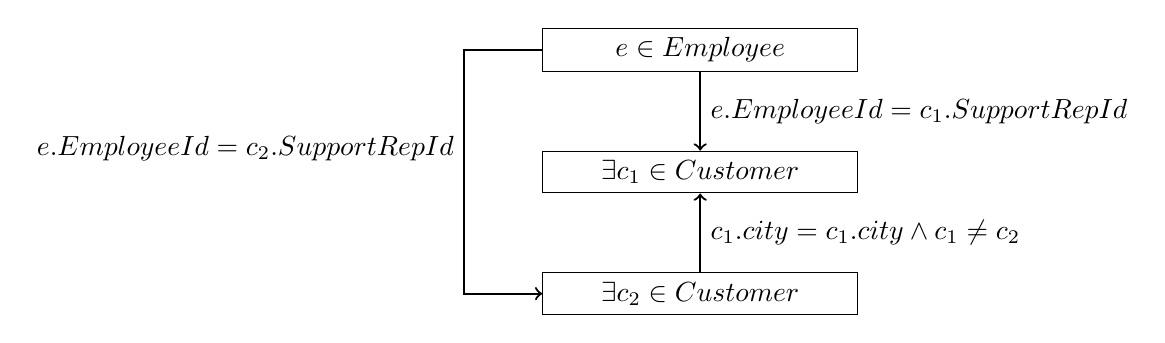
\begin{tikzpicture}[every node/.style={anchor=west, minimum width=4cm}]
			\node[draw, rectangle] (v1) {$e\in Employee$};
			
			\node[draw, rectangle, below = of v1] (v2) {$\exists c_1\in Customer$};
			
			\node[draw, rectangle, below = of v2] (v3) {$\exists c_2\in Customer$};
			
			\draw[->, thick,anchor=west] (v1) edge node {$e.EmployeeId = c_1.SupportRepId$} (v2) ;
			
			\draw[->, thick,anchor=west] (v3) edge node {$c_1.city=c_1.city \land c_1 \neq c_2$} (v2);
			
			\draw[->, thick, anchor = west] (v1) -| ++(-3,-0.125) node[pos=5.5, left]{$e.EmployeeId=c_2.SupportRepId$} |- (v3);
		\end{tikzpicture}
	\end{figure}

	This graph is cycle free, which means the query is optimizable using semi-joins.

	\subsection*{1.b)}
	$\{<t.name, t.composer> \mid t \in Track \land \exists g\in Genre \land g.GenreId=t.GenreId \land g.Name="Rock" \land \exists art\in Artist \land \exists alb \in Album \land alb.ArtistId=art.ArtistId \land t.AlbumId=alb.AlbumId \land t.Composer=art.Name\}$
	
	\begin{figure}[H]
		\centering
		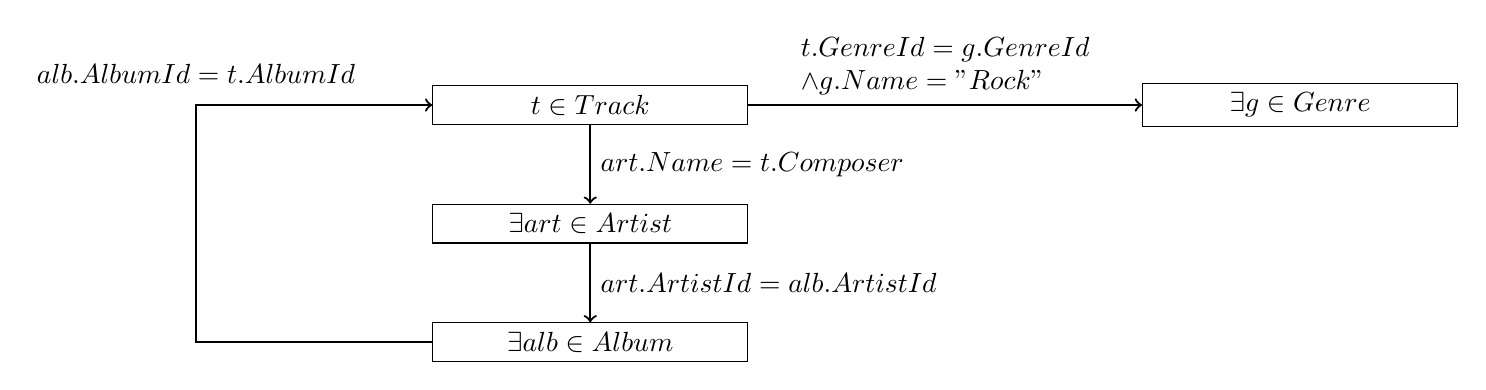
\begin{tikzpicture}[every node/.style={anchor=west, minimum width=4cm}]
		\node[draw, rectangle] (v1) {$t \in Track$};
		
		\node[draw, rectangle, right =5cm of v1] (v2) {$\exists g \in Genre$};
		
		\node[draw, rectangle, below = of v1] (v3) {$\exists art \in Artist$};
		
		\node[draw, rectangle, below = of v3] (v4) {$\exists alb \in Album$};
		
		\draw[->, thick,anchor=west, align =left] (v1) edge node[above] {$t.GenreId = g.GenreId$\\$ \land  g.Name="Rock"$} (v2) ;
		
		\draw[->, thick,anchor=east] (v1) edge node {$art.Name=t.Composer$} (v3);
		
		\draw[->, thick,anchor=west] (v3) edge node {$art.ArtistId=alb.ArtistId$} (v4);
		
		\draw[->, thick,anchor=west] (v4.west) -| ++(-3,0.35) node[pos = 5,above]{$alb.AlbumId=t.AlbumId$} |- (v1.west);
		\end{tikzpicture}
	\end{figure}

	This Graph has a cycle. This means the query is not optimizable using semi-joins.
	
	\subsection*{2.}
	$\{<t.Name> \mid t\in Track \land t.Miliseconds \le 90000 \land \exists g \in Genre \land t.GenreId=t.GenreId \land g.Name="Rock" \land \exists m\in MediaType \land t.MediaTypeId=m.MediaTypeid \land m.Name = "MPEG audio file"\}$
	
	\begin{figure}[H]
		\centering
		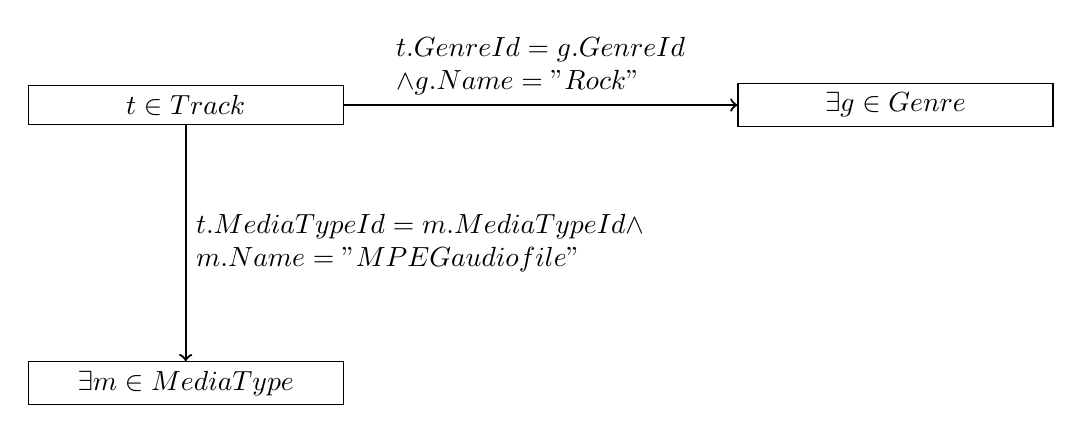
\begin{tikzpicture}[every node/.style={anchor=west, minimum width=4cm}]
		\node[draw, rectangle] (v1) {$t \in Track$};
		
		\node[draw, rectangle, right =5cm of v1] (v2) {$\exists g \in Genre$};
		
		\node[draw, rectangle, below = 3cm of v1] (v3) {$\exists m \in MediaType$};
		
%		\node[draw, rectangle, below = of v3] (v4) {$\exists alb \in Album$};
		
		\draw[->, thick,anchor=west, align =left] (v1) edge node[above] {$t.GenreId = g.GenreId$\\$ \land  g.Name="Rock"$} (v2) ;
		
		\draw[->, thick,anchor=east, align = left] (v1) edge node {$t.MediaTypeId = m.MediaTypeId \land$ \\ $m.Name="MPEG audio file"$} (v3);
		
		
		\end{tikzpicture}\\
		TODO: es fehlt das mit den $\le$90000ms %TODO
	\end{figure}
	The graph is cycle free, which means it can be optimized using semi-joins.
\end{document}


















